\documentclass[amsmath,amssymb,nofootinbib,prd]{article}
%\pdfoutput=1

%,superscriptaddress

\usepackage{graphicx}
\usepackage{float}
\usepackage{fullpage}
\usepackage[colorlinks=true,citecolor=blue]{hyperref}
\usepackage{dsfont}
\usepackage[utf8]{inputenc}
\usepackage[english]{babel}
\usepackage{mathtools}
\usepackage{amsmath}
\usepackage{bm}
\usepackage{braket}
\usepackage{latexsym}
\usepackage{amssymb}
\usepackage[compat=1.1.0]{tikz-feynman}
\usepackage{comment}


% new commands
\newcommand*\NewPage{\null\thispagestyle{empty}\newpage}
\DeclareUnicodeCharacter{00A0}{~}
\def \L{{\cal L}}
\def \({\left(}
\def \){\right)}
\def \[{\left[}
\def \]{\right]}
\newcommand{\tbf}[1]{{\textbf{#1}}}
\newcommand{\bsy}[1]{{\boldsymbol{#1}}}
\newcommand{\txt}[1]{\text{#1}}
\newcommand{\defeq}{\vcentcolon=}
\newcommand{\eqdef}{=\vcentcolon}
\newcommand{\cv}[1]{\underline{#1}}
\newcommand{\bQ}{{\textbf {Q}}}
\newcommand{\bq}{{\textbf {q}}}
% \newcommand{\bm}{{\textbf {m}}}
\newcommand{\br}{{\textbf {r}}}
\newcommand{\bU}{{\textbf {U}}}
\newcommand{\bu}{{\textbf {u}}}
\newcommand{\bV}{{\textbf {V}}}
\newcommand{\bF}{{\textbf {F}}}
\newcommand{\bY}{{\textbf {Y}}}
\newcommand{\bff}{{\textbf {f}}}
\newcommand{\bG}{{\textbf {G}}}
\newcommand{\bW}{{\textbf {W}}}
\newcommand{\bZ}{{\textbf {Z}}}
\newcommand{\bh}{{\textbf {h}}}
\newcommand{\bw}{{\textbf {w}}}
\newcommand{\bv}{{\textbf {v}}}
\newcommand{\bA}{{\textbf {A}}}
\newcommand{\bB}{{\textbf {B}}}
\newcommand{\bhx}{\hat {\textbf {x}}}
\newcommand{\bX}{{\textbf {X}}}
\newcommand{\bx}{{\textbf {x}}}
\newcommand{\bo}{{\textbf {o}}}
\newcommand{\blambda}{{\boldsymbol{\Lambda}}}
\newcommand{\btau}{{\boldsymbol{\tau}}}
\newcommand{\bsigma}{{\boldsymbol{\sigma}}}
\newcommand{\by}{{\textbf {y}}}
\newcommand{\bz}{{\textbf {z}}}
\newcommand{\bl}{{\textbf {l}}}
\newcommand{\bs}{{\textbf {s}}}
\newcommand{\bS}{{\textbf {S}}}
\newcommand{\bc}{{\textbf {c}}}
\newcommand{\bk}{{\textbf {k}}}
\newcommand{\bR}{{\textbf {R}}}
\newcommand{\beps}{{\boldsymbol {\epsilon}}}
\newcommand{\bxigma}{{\boldsymbol{\Sigma}}}
\newcommand{\bxi}{{\boldsymbol{\xi}}}
\newcommand{\bzero}{{\textbf{0}}}
\newcommand{\ba}{{\textbf {a}}}
\newcommand{\cC}{{\mathcal{C}}}
\newcommand{\cB}{{\mathcal{B}}}
\newcommand{\lab}[1]{\label{#1}}
\newcommand{\bxii}{{\boldsymbol{\xi}}}
\newcommand{\bre}{{\textbf {e}}}
\newcommand{\bytilde}{{\tilde{\textbf {y}}}}
\newcommand{\bxhat}{{\tilde{\textbf {x}}}}
\newcommand{\mc}{\mathcal}
\newcommand{\eps}{\varepsilon}
\newcommand{\calF}{\mathcal F}
\newcommand{\s}{\sigma}
\renewcommand{\d}{\text{d}}
\newcommand{\e}{\text {e}}
\newcommand{\ds}{\Delta\sigma}
\newcommand{\hw}{h^{\rm W}}
\newcommand{\sw}{\sigma^{\rm W}}
\newcommand{\<}{\langle}
\renewcommand{\>}{\rangle}
\newcommand{\de}{\partial}
\newcommand{\la}{\langle}
\newcommand{\ra}{\rangle}
\newcommand{\eq}{\text{ eq}}
\newcommand{\sign}{\text{ sign}}
\newcommand{\ua}{\uparrow}
\newcommand{\da}{\downarrow}
\newcommand{\be}{\begin{equation}}
\newcommand{\ee}{\end{equation}}
% \newcommand{\bea}{\begin{eqnarray}}
% \newcommand{\eea}{\end{eqnarray}}
\newcommand{\mE}{\mathbb{E}}
\newcommand\smallO{
  \mathchoice
    {{\scriptstyle\mathcal{O}}}% \displaystyle
    {{\scriptstyle\mathcal{O}}}% \textstyle
    {{\scriptscriptstyle\mathcal{O}}}% \scriptstyle
    {\scalebox{.7}{$\scriptscriptstyle\mathcal{O}$}}%\scriptscriptstyle
  }
\newcommand{\bea}{\begin{align}}
\newcommand{\eea}{\end{align}}

\newtheorem{theorem}{Theorem}[section]
\newtheorem{lemma}[theorem]{\textbf{Lemma}}
\newtheorem{thm}[theorem]{\textbf{Theorem}}
\newtheorem{remark}[theorem]{\textbf{Remark}}
\newtheorem{proposition}[theorem]{\textbf{Proposition}}
\newtheorem{corollary}[theorem]{\textbf{Corollary}}
\newtheorem{definition}[theorem]{\textbf{Definition}}


\DeclareMathOperator{\atanh}{atanh}
\DeclareMathAlphabet{\varmathbb}{U}{bbold}{m}{n}
\newcommand{\id}{\mathds{1}}
\newcommand{\EE}{\mathbb{E}}
\newcommand{\noi}{\noindent}
\renewcommand{\d}{{\rm d}}
\renewcommand{\P}{{\rm P}}
% \newcommand{\eq}[1]{\begin{align}#1\end{align}}
\newcommand{\B}{{\rm B}}
\newcommand{\Tr}{{\rm Tr}}
\newcommand{\iif}{\Longleftrightarrow}
\newcommand{\bbR}{\mathbb{R}}
% \newcommand{\bF}{{\bf{F}}}
% \newcommand{\bx}{{\bf{x}}}
%

\begin{document}

\title{The Kac-Rice formula: basic definitions and a first application}
\date{\today}
\author{Antoine Maillard}
\maketitle
%
\renewcommand{\labelitemi}{$\bullet$}

These notes are based on a brief introduction given at the Kavli Institute for Theoretical Physics (Santa Barbara) in February 2019.

\section{The Kac-Rice formula}

\subsection{The area formula}
	The Kac-Rice formula is intuitively not derived from any involved probabilistic tool, but rather is a consequence of a purely geometric result, called the area formula (itself a consequence of the more general corea formula), described in much more generality by Federer \cite{federer1959curvature}, and stated for instance in \cite{azais2009level}. 
	This formula is the generalization of the following non-rigorous intuition: for a smooth function $f : \bbR \to \bbR$, and $T \subseteq \bbR$,
	 denoting $N_f(u,T)$ the number of solutions to the equation $f(t) = u$ with $t \in T$, one would want to write informally:
	\begin{align}
	N_f(u,T) &= \int_{f(T)} \delta\left(v - u\right) \mathrm{d}v, \\
	\label{eq:area_informal}
	  &= \int_T \delta\left(f(t) - u\right) |f'(t)| \mathrm{d}t.
	\end{align}
	The area formula generalizes and makes rigorous this intuition, by showing a weak version of this last equality. We follow here the statement of \cite{azais2009level}. 
	\begin{proposition}[Area formula]\label{prop:area}
	Let $f : U \to \bbR^d$ be a $\mathcal{C}^1$ function defined on an open subset $U$ of $\bbR^d$. Assume that the sets of critical values of $f$ has zero Lebesgue measure, and denote $N_f(u,T)$  the number of solutions to the equation $f(t) = u$ with $t \in T$. Then, for any Borel set $T \subset \bbR^d$, and any $g : \bbR^d \to \bbR$ continuous and bounded:
	\begin{align}
\int_{\bbR^d} g(u) N_f(u,T) &= \int_T \, \left|\det f'(t)\right| \, g(f(t)) \,\mathrm{d}t. 	
	\end{align}
	\end{proposition}
	Note that in a large part of the theoretical physics literature, the area formula (and subsequently the Kac-Rice formula) is written in the form of eq.~\eqref{eq:area_informal}, 
	without further considerations.
	
	\subsection{Informal derivation of Kac-Rice}
	
	Consider a smooth compact manifold $\mathcal{M}$ of dimension $n$ (think of the unit sphere in $n$ dimensions $\mathbb{S}^{n-1}$), equipped with a Riemannian metric, and an associated volume measure $\mu_{\mathcal{M}}$. 
	We are given a random smooth function $f : \mathcal{M} \to \bbR$. 
	We want to use the area formula (Proposition~\ref{prop:area}) to estimate the moments of the number of critical points of $f$.  
	Given the hypotheses of Proposition~\ref{prop:area}, a reasonable hypothesis is to assume that $f$ is almost surely a \emph{Morse} function, i.e.\ that \emph{all its critical points are non-degenerate}. 
	Since $\mathcal{M}$ is compact, one easily deduces that the number of critical points of a Morse function is finite\footnote{Note that the numbers of critical points of different indices of a Morse function are constrained by the topology of $\mathcal{M}$ by the Morse inequalities, see \cite{milnor1963morse} for a review on Morse theory.}. 
	For any $k \in \mathbb{N}$ and Borel set $B \subseteq \bbR$, we define $\mathrm{Crit}_{f,k}(B)$ to be the number of critical points $x \in \mathcal{M}$ of $f$ such that $f(x) \in B$
	 and such that the index of $\mathrm{Hess}\, f(x)$ (that is the number of strictly negative eigenvalues of the Hessian) is equal to $k$. 
	 The informal area formula of eq.~\eqref{eq:area_informal}, applied to $\mathrm{grad}\ f$, would read:
	\begin{align}
	\mathrm{Crit}_{f,k}(B) &= \int_{\mathcal{M}} \mathrm{d}\mu_{\mathcal{M}}(x) \delta\left(\mathrm{grad}\, f(x)\right) \left|\det \, \mathrm{Hess}\, f(x)\right| \, \mathds{1}\left[f(x) \in B,\, \mathrm{i}\left(\mathrm{Hess}\, f(x)\right) = k\right]
	\end{align}
	Taking the expectation of this equality, one directly obtains the Kac-Rice formula:
	\begin{proposition}[Kac-Rice formula, informal]\label{prop:KR}Let $\mathcal{M}$ be a smooth compact Riemannian manifold of dimension $n$, with volume measure $\mathcal{\mu}_M$. Let $f : \mathcal{M} \to \bbR$ be a random function 
		that is almost surely Morse.
		Denote  $\varphi_{\mathrm{grad}\, f(x)}(0)$ the density of $\mathrm{grad}\, f(x)$ with respect to the Lebesgue measure on $\bbR^{n-1}$, taken at $0$. Then:
	\begin{align*}
	\EE \, \mathrm{Crit}_{f,k}(B) &= \int_{\mathcal{M}} \mathrm{d}\mu_{\mathcal{M}}(x) \EE \left[\left|\det \, \mathrm{Hess}\, f(x)\right| \, \mathds{1}\left[f(x) \in B,\, \mathrm{i}\left(\mathrm{Hess}\, f(x)\right) = k\right] \middle| \mathrm{grad}\, f(x) = 0 \right] \varphi_{\mathrm{grad}\, f(x)}(0).
	\end{align*}
	\end{proposition}\vspace{0.cm}
	
	\paragraph{Some remarks}:
	\begin{enumerate}
	\item The rigorous derivation of this formula is much more involved, as one has to start from the weak equality of Proposition~\ref{prop:area} and to use continuity arguments in order to obtain an equality at $u = 0$, see for instance the proof of Kac-Rice performed in \cite{azais2009level}.
	This is the first reason for which the formula is usually stated for Gaussian random fields, since in these cases these continuity arguments can be justified using simple hypotheses on the covariance of the random field.
	The second reason is that in general, conditional expectations of non-Gaussian random variables are intractable, making the Kac-Rice formula effectively useless since one has to know the law of the Hessian conditioned by the gradient being zero.
	 Under many heavy technical conditions, one can however derive rigorous non-Gaussian versions of the Kac-Rice formula, see for example Theorem~12.1.1 of \cite{adler2009random} and Theorem~6.7 of \cite{azais2009level}.
	\item The Kac-Rice formula transforms a random differential geometry problem into a random matrix theory problem.
	This does not necessarily mean that the resulting problem will be simpler !
	The main difficulty in evaluating the Kac-Rice formula comes from the distribution of the Hessian conditioned by the gradient being zero.
	% Even for Gaussian random fields, this is in general a heavily correlated Gaussian random matrix, for which very few results exist. 
	\item The Kac-Rice formula can be generalized to compute higher moments of the variable $\mathrm{Crit}_{f,k}(B)$ as well (see Theorem~6.3 of \cite{azais2009level}), and can therefore be used to compute the second moment of the complexity (see \cite{subag2017complexity} for an application to the pure spherical $p$-spin model) as well as perform heuristic replica calculations to obtain the quenched complexity (see for instance \cite{ros2019complex}).
	Via Morse's theory, it can also be used to compute the moments of the Euler characteristic of the level sets of $f$, see \cite{auffinger2013complexity} for an example.
	\end{enumerate}
	
	\section{The annealed complexity of the pure spherical \texorpdfstring{$p$}{p}-spin model}
	
	We essentially detail here a calculation performed first by physicists, and made rigorous in \cite{auffinger2013random}. 
	We follow here the derivation of this last paper. For (anterior) theoretical physics derivation of the complexity of similar models using the Kac-Rice formula along with heuristic theoretical physics arguments (giving nevertheless the exact result), one can for instance read the works of Fyodorov: \cite{fyodorov2004complexity}, \cite{fyodorov2007replica}. 
	
	\subsection{Statement of the problem}
	Consider $N \geq 1$, $p \geq 3$, and consider the following function $f_{N,p}$ on the unit sphere $\mathbb{S}^{N-1}$:
	\begin{align}
	f_{N,p}(\bsigma) &\triangleq \sum_{1 \leq i_1,\cdots,i_p \leq N} J_{i_1,\cdots i_p} \bsigma_{i_1} \cdots \bsigma_{i_p} \hspace{1cm} (\bsigma \in \mathbb{S}^{N-1}) ,
	\end{align}
	in which $J_{i_1,\cdots i_p} \overset{\mathrm{i.i.d.}}{\sim} \mathcal{N}(0,1)$.
	In the physics language, the Hamiltonian $H_{N,p}$ of the spherical $p$-spin model (defined on $\mathbb{S}^{N-1}(\sqrt{N})$), is related to $f_{N,p}$ by: $f_{N,p}(\bsigma) = \frac{1}{\sqrt{N}} H_{N,p}(\sqrt{N}\bsigma)$.
	For any Borel set $B \subseteq \bbR$, we want to compute the large $N$ limit of the expectation of the number of local minima $\bsigma$ of $f_{N,p}$, such that $f_{N,p}(\bsigma) \in \sqrt{N} B$, tha we denote $\mathrm{Crit}_{N,p}^0(B)$,. 
	One can apply the Kac-Rice formula (Proposition~\ref{prop:KR})\footnote{The proof that $f_{N,p}$ is almost surely a Morse function can be found in \cite{auffinger2013random}}:
	\begin{align*}
	\EE \, \mathrm{Crit}_{N,p}^0(B) = \int_{\mathbb{S}^{N-1}} \mathrm{d}\mu(\bsigma) &\varphi_{\mathrm{grad}\, f_{N,p}(\bsigma)}(0)  \\ 
	&\EE \left[\left|\det \, \mathrm{Hess}\, f_{N,p}(\bsigma)\right| \, \mathds{1}\left[f_{n,p}(\bsigma) \in \sqrt{N} B,\, \mathrm{Hess}\, f_{N,p}(\bsigma) \geq 0\right] \middle| \mathrm{grad}\, f_{N,p}(\bsigma) = 0 \right],
	\end{align*}
	in which $\mu$ is the usual surface measure on $\mathbb{S}^{N-1}$. Note that here $\mathrm{grad}$ and $\mathrm{Hess}$ denote the \emph{Riemannian} gradient and Hessian on the sphere, while we will denote $\nabla$, $\nabla^2$ the Euclidian gradient and Hessian. 
	
	\subsection{The joint distribution of \texorpdfstring{$(f(\bsigma),\mathrm{grad}\, f(\bsigma),\mathrm{Hess}\, f(\bsigma))$}{(f,grad f, Hess f)}}
	
	Deriving the joint law of $(f(\bsigma),\mathrm{grad}\, f(\bsigma),\mathrm{Hess}\, f(\bsigma))$ is a necessary step in the Kac-Rice method, as these three 
	random variables appear in the conditional expectation.
	We fix $\bsigma  \in \mathbb{S}^{N-1}$. 
	In our case, it is immediate that the random variable $(f(\bsigma),\mathrm{grad}\, f(\bsigma),\mathrm{Hess}\, f(\bsigma))$ is a Gaussian centered random variable, as the sum of independent Gaussian centered random variables.
    We thus simply need to compute its correlations to fully characterize their joint distribution. We naturally identify the tangent space $\mathcal{T}_\bsigma(\mathbb{S}^{N-1})$ with $\bbR^{N-1}$. If we denote $P_\bsigma^\perp$ the orthogonal projector on $\{\bsigma\}^\perp$, one has:
	\begin{align}
	\mathrm{grad}\, f(\bsigma) &= P_\bsigma^\perp \nabla f(\bsigma), \\
	\mathrm{Hess}\, f(\bsigma) &= P_\bsigma^\perp \nabla^2 f(\bsigma) P_{\bsigma}^\perp - \braket{\bsigma,\nabla f(\bsigma)} P_\bsigma^\perp.
	\end{align}
	For instance one can compute the covariance of the gradient:
	\begin{align*}
	\EE \left[\mathrm{grad}\, f(\bsigma) \mathrm{grad}\, f(\bsigma)^\intercal \right] &=  P_\bsigma^\perp\EE \left[\nabla f(\bsigma) \nabla f(\bsigma)^\intercal \right] P_\bsigma^\perp, \\
	&= p  P_\bsigma^\perp.
	\end{align*}
	Uisng the same kind of simple algebraic calculations, one obtains the joint distribution:
	\begin{lemma}\label{lemma:joint}
	The joint law of $(f(\bsigma),\mathrm{grad}\, f(\bsigma),\mathrm{Hess}\, f(\bsigma))$ is the following:
	\begin{align}
	\begin{cases}
	f(\bsigma) &\overset{d}{=} Z, \\
	\mathrm{grad}\, f(\bsigma) &\overset{d}{=} \sqrt{p} \bm{g}, \\
	\mathrm{Hess}\, f(\bsigma) &\overset{d}{=} \sqrt{2 (N-1)p(p-1)} M_{N-1} - p Z \, \mathrm{Id}_{N-1},
	\end{cases}
	\end{align}
	in which $Z \sim \mathcal{N}(0,1)$, $\bm{g} \sim \mathcal{N}(0,\mathrm{Id}_{N-1})$, and $M_{N-1}$ is a matrix from the Gaussian Orthogonal Ensemble of size $(N-1)$ with the convention $\EE M_{ij}^2 = \frac{1+\delta_{ij}}{2(N-1)}$. The variables $(Z,\bm{g},M_{N-1})$ are pairwise independent.
	\end{lemma}
	Let us make the following important remarks:
	\begin{enumerate}
	\item The joint distribution of these variables is independent of $\bsigma$.
	\item The variables $(f,\mathrm{Hess}\, f)$ are independent from $\mathrm{grad}\,f$, so performing the conditioning in the Kac-Rice formula will be trivial.
	\item From the gradient distribution, one easily obtains its density evaluated in $0$:
	\begin{align*}
	 \varphi_{\mathrm{grad}\, f_{N,p}(\bsigma)}(0) &= e^{- \frac{N-1}{2} \ln (2 \pi p)}.
	\end{align*}
	\end{enumerate}
	Recalling that the volume of the unit sphere is $V(\mathbb{S}^{N-1}) = 2 \pi^{N/2} / \Gamma(N/2)$, one deduces from the Kac-Rice formula and what we said above:
	\begin{align}\label{eq:0}
	\EE \, \mathrm{Crit}_{N,p}^0(B) &= \frac{2 \pi^{N/2}}{\Gamma(N/2)}e^{- \frac{N-1}{2} \ln (2 \pi p)} \left[2 (N-1)p(p-1)\right]^{\frac{N-1}{2}} \EE \left[|\det H_{N-1}| \mathds{1}(H_{N-1} \geq 0, \, z \in \sqrt{N} B)\right],
	\end{align}
	in which $H_{N-1} \triangleq M_{N-1} - \sqrt{\frac{p}{2 (N-1)(p-1)}} z$, with $z$ a standard Gaussian variable and $M_{N-1}$ a GOE matrix of size $N-1$ (see Lemma~\ref{lemma:joint}), independent of $z$. 
	It is now completely clear that we reduced a random differential geometry problem (counting the number of critical points of a random smooth function) to a random matrix theory problem. 
	
	\subsection{Simplification of the problem}
	
	It is clear from eq.~\eqref{eq:0} that the following lemma (from \cite{auffinger2013random}) will be useful:
	\begin{lemma}\label{lemma:simplification} Let $G \subseteq \bbR$ a Borel set, $X \sim \mathcal{N}(0,t^2)$ (for a $t > 0$) and $M_{N-1} \sim \mathrm{GOE}(N-1)$. Then:
	\begin{align}
	\EE &\left[|\det (M_{N-1} - X \mathrm{Id}_{N-1})| \mathds{1}( (M_{N-1} - X \mathrm{Id}_{N-1}) \geq 0, X \in G)\right] \nonumber \\
	&\qquad = \frac{\Gamma\left(\frac{N}{2}\right)(N-1)^{-\frac{N}{2}}}{\sqrt{\pi t^2}} \EE_{\mathrm{GOE}(N)} \left[e^{-\frac{N}{2}\left(\frac{1}{(N-1)t^2} - 1\right) \lambda_0^2} \mathds{1} \left(\lambda_0 \in \sqrt{\frac{N-1}{N}} G\right)\right].
	\end{align}
	In this equation, $\lambda_0$ is the smallest eigenvalue of a random matrix from the GOE$(N)$ ensemble. 
	\end{lemma}
	This lemma is a pure result of random matrix theory.
	We do not prove it here, as it is proven as a particular case of Lemma~3.3 of \cite{auffinger2013random}.
	The idea of the proof is to write explicitly the joint law of the eigenvalues of $M_{N-1}$, denoted $\lambda_1 \leq \cdots \leq \lambda_{N-1}$, and to interpret $X$ as the smallest eigenvalue of a larger $\mathrm{GOE}(N)$ matrix with eigenvalues $X \leq \lambda_1 \leq \cdots \leq \lambda_{N-1}$, and use Selberg's integral. 
	Applying this lemma to eq.~\eqref{eq:0} with $t = \sqrt{\frac{p}{2 (N-1)(p-1)}}$ and  $G = (t\sqrt{N}) B$ yields that for any $N$:
	\begin{align}\label{eq:1}
	\EE \, \mathrm{Crit}_{N,p}^0(B) &= 2 \sqrt{\frac{2}{p}} (p-1)^{\frac{N}{2}} \EE_{\mathrm{GOE}(N)} \left[e^{-N \frac{p-2}{2p} \lambda_0^2} \mathds{1} \left(\lambda_0 \in  \sqrt{\frac{p}{2(p-1)}} B\right)\right].
\end{align}		
	
	\subsection{The large \texorpdfstring{$N$}{N} limit}
	
	We are interested in the limit of the annealed complexity $\Sigma^0_p(B) \triangleq \lim_{N \to \infty} \frac{1}{N} \ln \EE \, \mathrm{Crit}_{N,p}^0(B)$. 
	A precise look at eq.~\eqref{eq:1} can convince that we need to study the large deviations for the smallest eigenvalue of a $\mathrm{GOE}(N)$ matrix. We state this result in an informal way, see Theorem~A.1 of \cite{auffinger2013random} for a more precise statement, along with the Large Deviation Principle (LDP) for eigenvalues of all finite index:
\begin{lemma}[LDP of the smallest eigenvalue of a GOE matrix, informal]\label{lemma:ldp}
Let $\lambda_0$ be the smallest eigenvalue of a $\mathrm{GOE}(N)$ matrix, and $I \subseteq \bbR$. Then
\begin{align}
\lim_{N \to \infty} \frac{1}{N} \ln \mathbb{P}\left[\lambda_0 \in I\right] &= - \sup_{x \in I} F(x),
\end{align}
with $F$ defined as:
\begin{align}
F(x) &\triangleq \begin{cases} \infty &\mathrm{if}\,x \geq -\sqrt{2}  \\
 \frac{1}{\sqrt{2}} \int_{\sqrt{2}}^{-x} \mathrm{d}z\sqrt{\frac{z^2}{2} -1} & \mathrm{otherwise}
\end{cases}.
\end{align}
\end{lemma}
Using Lemma~\ref{lemma:ldp} alongside eq~\eqref{eq:1} and Varadhan's lemma directly yields a final estimate for the annealed complexity:
\begin{align}\label{eq:2}
\Sigma_p^0(B) &= \frac{1}{2} \ln (p-1) + \sup_{x \in \sqrt{\frac{p}{2(p-1)}} B} \left[-\frac{p-2}{2p}x^2 - F(x)\right].
\end{align}
	
\subsection{Description of the results}\label{subsec:summary}

Considering $B = (-\infty,u)$ (for $u \in \bbR$) in eq.~\eqref{eq:2} leads to effectively count the local minima of the pure $p$-spin Hamiltonian of extensive energy smaller than $Nu$. 
In this case, the supremum in eq.~\eqref{eq:2} can be analytically performed, and one obtains an explicit form for $\Sigma_p^0((-\infty,u))$.
The calculation we sketched can also be performed for critical points of any fixed index $k \in \mathbb{N}$ (see again \cite{auffinger2013random}), and if we define:
\begin{align}
\Theta_k(u) \triangleq \lim_{N \to \infty} \frac{1}{N} \ln \EE \, \mathrm{Crit}_{N,p}^k((-\infty,u)),
\end{align}
there exists analytic expressions for all $\Theta_k(u)$ functions, see eq~(2.16) of \cite{auffinger2013random}. 
Defining the \emph{threshold} energy $E_\infty \equiv 2 \sqrt{\frac{p-1}{p}}$, we can sketch the plot of these functions, see Fig.~\ref{fig:fig}.
We also denote $-E_k$ the value at which the function $\Theta_k(u)$ becomes positive.
	\begin{figure}
	\centering
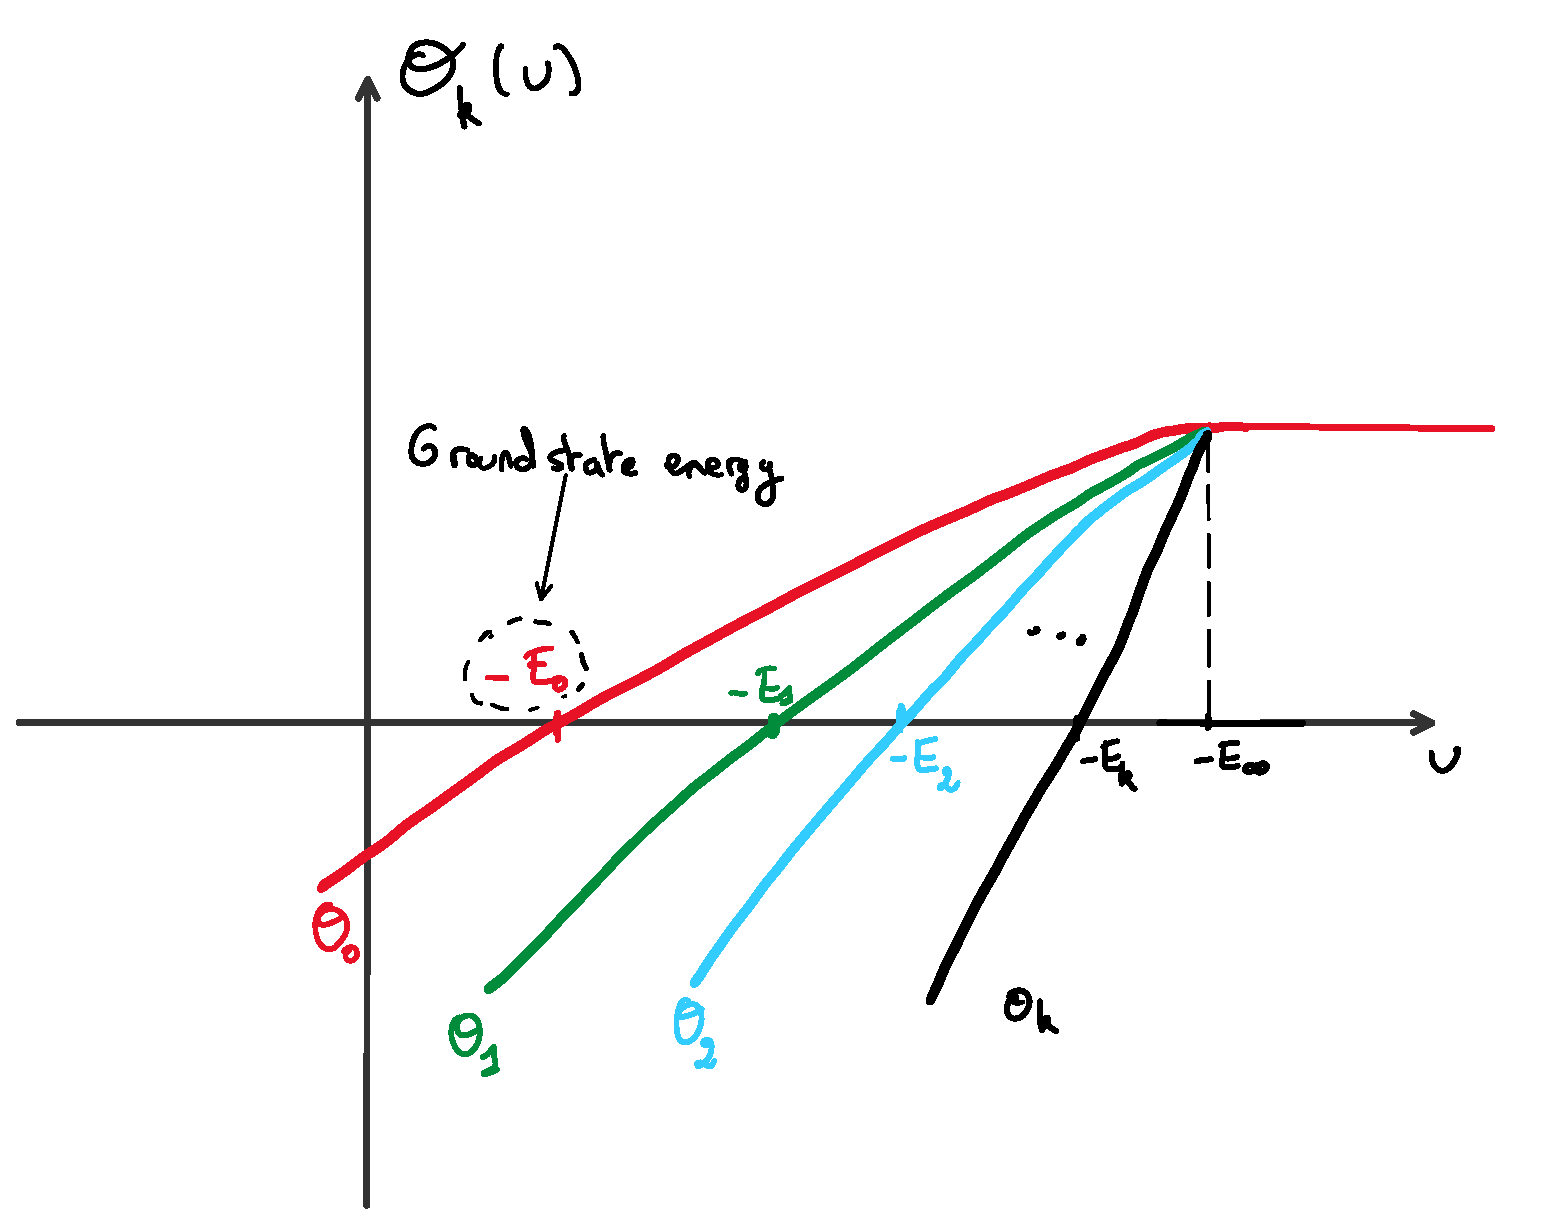
\includegraphics[scale=0.4]{figure.pdf}
\caption{The functions $\Theta_k$ for the first indices}\label{fig:fig}
\end{figure}

\paragraph{Final remarks}
\begin{enumerate}
\item The local minima always dominate the complexity for all energies below $-N E_\infty$, while for all energies above $-N E_\infty$, the complexity is dominated by critical points of diverging index.
\item The value $-E_0$ is the lowest energy of critical points, and corresponds to the global minimum of the original function.
It can be shown indeed (\cite{auffinger2013random}) that the ground state energy concentrates to a deterministic value as $N \to \infty$.
\item One can perform similar calculations for the complexity of critical points whose indices diverge with $N$, see \cite{auffinger2013complexity}  for the rigorous derivation.
\item This rigorous calculation can also be generalized to the mixed spherical $p$-spin case, see again \cite{auffinger2013complexity}. 
By a classical result of Schoenberg, these models exhaust all stationary isotropic Gaussian random fields on the sphere in $N$ dimensions.
\end{enumerate}

\bibliographystyle{alpha}
\bibliography{refs}
\end{document}
	